%Tech Science Press -- CMC submission
%=================================================================
\documentclass[cmc,article,submit,moreauthors,pdftex]{Definitions/tsp}
\input{Definitions/package}
\input{Definitions/unicode}

%=================================================================
% Internal commands: Article information and pagination will be assigned by the Editorial Office
\continuouspages{}
\firstpage{1}
\makeatletter
\setcounter{page}{\@firstpage}
\makeatother
\pubvolume{0}
\issuenum{0}
\elocationid{0}
\articlenumber{0}
\pubyear{2026}
\copyrightyear{2026}
\datereceived{Day Month Year}
\dateaccepted{Day Month Year}
\dateonlinefirst{}
\datepublished{Day Month Year}

%=================================================================
\usepackage{algorithmic}
\newcommand{\cges}{C\textsuperscript{2}GES}
\newcommand{\adot}{.} % protected dot for arXiv identifiers in the bibliography (vancouver.bst strips plain dots from journal fields)

%=================================================================
% Full title of the paper (Capitalized)
\Title{Causal-Role-Aware Extractive Evidence Selection for Power Grid Reliability Reports}

% Authors, for the paper (add full first names)
\Author{Bijing Liu\textsuperscript{1,2} and Yong Yang\textsuperscript{1,2,*}}

% Authors, for metadata in PDF
\AuthorNames{Bijing Liu and Yong Yang}

% Affiliations / Addresses (Add [1] after \address if there is only one affiliation.)
\address{%
\textsuperscript{1}NARI Group Corporation (State Grid Electric Power Research Institute), Nanjing 211106, Jiangsu Province, China

\textsuperscript{2}Beijing Kedong Electric Power Control System Co., Ltd., Beijing 100080, China
}%

% Contact information of the corresponding author
\corres{Corresponding Author: Yong Yang. Email: yangyong1@sgepri.sgcc.com.cn}

% Abstract (Do not use inserted blank lines, i.e. \\)
\abstract{Power-grid reliability reports contain causal event narratives whose supporting evidence is dispersed across technical prose. This paper formulates report review as causal-role-conditioned sentence-ID selection and introduces \cges{}, a deterministic reranker combining query relevance, role compatibility, and a role-selective local chain signal. The benchmark contains 40 public North American Electric Reliability Corporation reports or excerpts and 200 five-role questions. To test label sensitivity, 75 questions from a frozen 15-document subset were independently reannotated by three AI agents configured as complementary simulated experts; they were blinded to the original answers, labels, cue lexicons, and model outputs. Sentence-level majority adjudication required no fallback, any annotator pair exactly agreed on 86.7\% of questions, and pairwise binary sentence Cohen's $\kappa$ ranged from 0.792 to 0.834. These annotations are explicitly not human-gold labels. Replacing the corresponding 75 labels yields a mixed-provenance 200-question benchmark on which \cges{} reaches 0.2882 evidence F1, compared with 0.1987 for TF-IDF, 0.2213 for BM25, and 0.1851 for SBERT; the document-cluster bootstrap difference over BM25 is $+0.0669$ (95\% confidence interval $[0.0325,0.1000]$, $p<0.001$). The frozen 75-question reannotated subset provides a stricter robustness check: \cges{} reaches 0.2719 F1, essentially matching BM25 (0.2712), trailing BGE and cross-encoder rerankers (0.3035 and 0.3155), and substantially trailing a zero-shot LLM selector (0.5699). On that subset, the no-role ablation reaches 0.2641 and the full-versus-TF-IDF confidence interval crosses zero. Thus, the original aggregate role-aware gain is not independently confirmed by the simulated-expert subset. The contribution is consequently bounded to an auditable deterministic reranker, a fully disclosed mixed-provenance benchmark, and an annotation-sensitivity analysis that exposes where conclusions do and do not survive label revision; real dual-expert human annotation remains required before the benchmark can be called human-gold.}

% List 3 to 10 pertinent keywords specific to the article
\keyword{Extractive summarization; causal evidence selection; power grid maintenance reports; NERC reliability reports; causal-role reranking; evidence retrieval}

%%%%%%%%%%%%%%%%%%%%%%%%%%%%%%%%%%%%%%%%%%%
\begin{document}

\section{Introduction}
\label{sec:introduction}

Power-grid maintenance and reliability reports preserve operational knowledge about disturbances, protection actions, equipment behavior, remediation, and lessons learned. In this paper, the phrase ``maintenance reports'' is used broadly to refer to public NERC reliability, disturbance, lessons-learned, and event-focused report excerpts that document grid events and corrective actions. Their value lies not only in the events they describe, but in the causal mechanisms that connect a triggering condition to a downstream operational impact and an eventual mitigation. Such reports are used in post-event review, where traceable sentences can support claims about causes, impacts, protection behavior, operator response, and corrective actions. This requirement is sharpened by the growing role of data-driven analysis in electric power systems, where AI methods are increasingly discussed for grid modeling, reliability, forecasting, and digital infrastructure, but where textual evidence from reports remains difficult to operationalize \cite{xie2022massively,srinivasan2023artificial,hamann2024foundation,madabhushi2023survey}. \cges{} studies this problem as evidence-grounded causal-role sentence selection: given NERC report sentences and a causal role question, the system returns evidence sentence IDs. This formulation follows the spirit of query-focused summarization benchmarks such as QMSum, where the information need conditions the relevant content, but adapts the unit of prediction to sentence-level causal evidence rather than a fluent generated answer \cite{zhong2021qmsum}. Building on this observation, the paper treats selected evidence as the primary model output and treats any downstream causal summary as a packaging layer over that selected evidence.

Generic extractive summarization and generic retrieval leave a gap for this setting because relevance alone does not determine causal role. A sentence describing load loss may be central to an event narrative, but it may answer an impact question rather than a root-cause question; similarly, a sentence mentioning relay operation may describe propagation, mitigation, or both depending on its local context. Classical and modern extractive summarization methods rank sentences by salience, centrality, redundancy control, or learned sentence matching \cite{zhong2020extractive,bi2021aredsum,joshi2022ranksuman}. Graph-based summarizers extend this idea by modeling sentence or heterogeneous document structure, including TextRank-style ranking, heterogeneous graph neural networks, and multiplex sentence graphs \cite{khor2021text,wang2020heterogeneous,jing2021multiplex,cui2020enhancing}. Query-focused systems instead condition selection or generation on an explicit information need, and recent work has examined query-focused meeting summarization, salient-content ranking, and evidence attribution for long-context summarization \cite{vig2022exploring,liu2023rank,sotudeh2024rank,wright2025unstructured}. In contrast to these broader summarization settings, NERC report analysis requires distinguishing among causal roles that are topically close but operationally different. The benchmark therefore asks whether role-conditioned evidence selection improves over lexical query retrieval, semantic query retrieval, positional baselines, and graph-centrality summarization baselines on the same sentence pools.

Causal language further complicates the task because causal terms in text are suggestive but insufficient for operational event reconstruction. Prior work in causal NLP has emphasized that extracting, representing, or reasoning about causal relations requires care about what is being estimated or inferred \cite{feder2022causal,kcman2023causal,gao2023chatgpt,wang2024causalbench}. Other work has studied explainable causal reasoning datasets, procedural causal event reasoning, document-level causal relation extraction, and causal structure induction for summarization \cite{du2022ecare,zhang2023causal,wang2024documentlevel,chen2023inducing}. These directions motivate causal-role awareness, but the present task is narrower: it evaluates whether a reranker can recover annotated evidence sentences for role-specific questions in public power-grid reports or report excerpts. The ``counterfactual'' terminology in \cges{} is correspondingly scoped to ablation-style component removal. By removing scoring components, the experiments ask what changes when role compatibility or chain consistency is absent, rather than simulating alternative physical grid trajectories or estimating structural causal effects. This scope matters because power-system disturbances involve protection settings, operator actions, equipment states, and regional grid behavior that are not fully recoverable from report prose alone.

\cges{} is a lightweight reranking method for this role-conditioned evidence task. For each document sentence, question, and causal role, \cges{} combines a query relevance score with a role compatibility score and a local causal-chain consistency score. Query relevance supplies the retrieval backbone, role compatibility biases the ranker toward sentences that express the requested causal function, and chain consistency is activated only for propagation/response and mitigation questions, where nearby causal-mechanism context is most likely to affect the selected evidence. Fig.~\ref{fig:architecture_overview} gives an overview of the architecture. The method is implemented as a sentence ranker over the local benchmark at \path{verification_pilot/agent_audit_40doc/}, with the post-freeze revision package under \path{post_freeze_revisions/role_selective_graph_gate/}; the Executor revision records completed metrics in the run artifact used for this revised manuscript. The empirical pattern is clear on the candidate benchmark: the full method outperforms lexical and semantic query retrieval, and the role ablation identifies causal-role compatibility as the dominant source of the improvement. The graph term remains auxiliary but measurable in the role-selective revision, which turns the main technical message toward scoped role-aware reranking with a small structural adjustment rather than broad graph inference.

\begin{figure}[!ht]
\centering
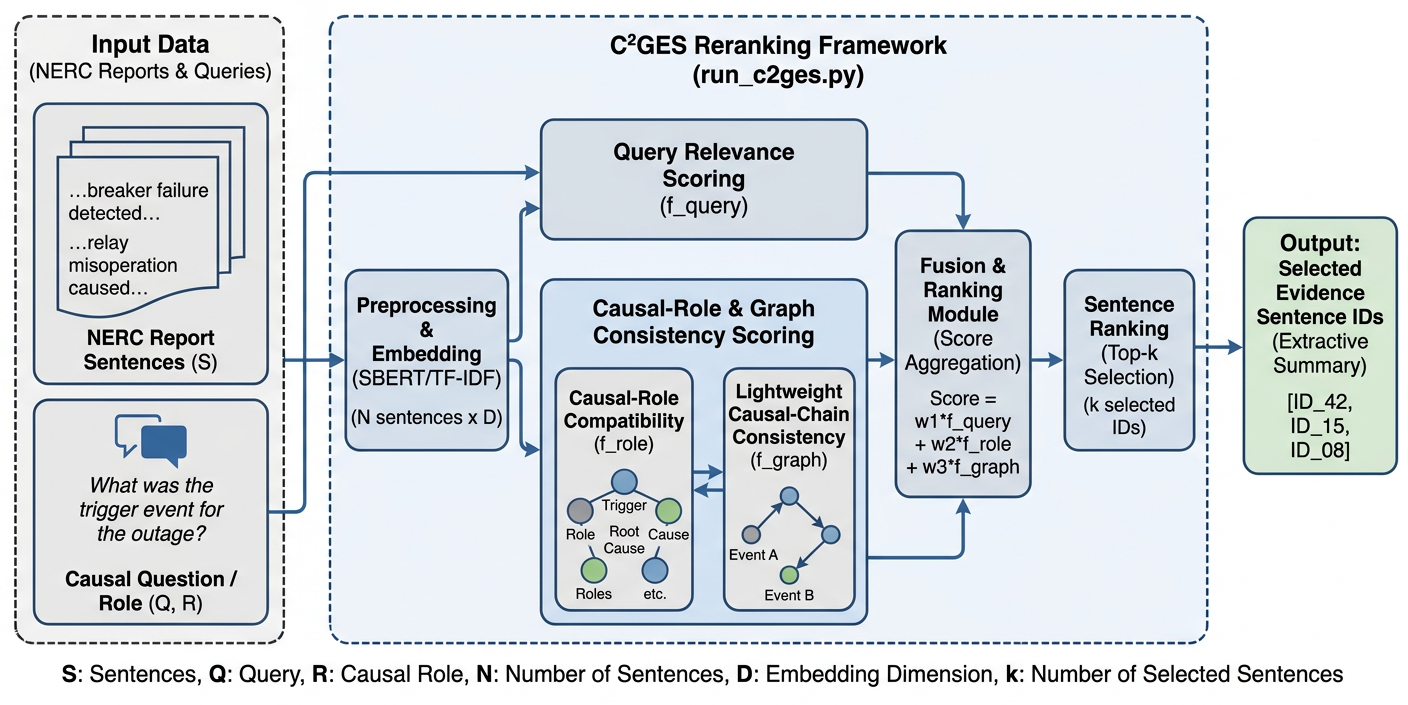
\includegraphics[width=0.72\textwidth]{charts/architecture_diagram_1.png}
\caption{Overview of the \cges{} architecture. For each report sentence, question, and causal role, the reranker combines query relevance, role compatibility, and a role-selective causal-chain consistency signal into an additive score and emits the top-$K$ evidence sentence IDs.}
\label{fig:architecture_overview}
\end{figure}

This paper makes three contributions:
\begin{itemize}
  \item It defines an evidence-grounded causal-role selection benchmark over public NERC reports and excerpts and releases a versioned mixed-provenance revision in which a frozen 75-question subset is replaced by majority-adjudicated labels from three blinded AI simulated-expert annotators.
  \item It introduces \cges{} as a lightweight causal-role-aware reranker for the task of mapping NERC report sentences and a causal-role question to evidence sentence IDs, with role-selective graph consistency framed as an auxiliary chain-consistency feature rather than as full graph neural inference or power-system simulation.
  \item It evaluates \cges{} against lexical, neural, and LLM rerankers under both the mixed 200-question benchmark and the reannotated 75-question subset, showing that the aggregate role-aware gain persists only in the mixed benchmark and is not independently confirmed on the simulated-expert subset.
\end{itemize}

The rest of this paper is organized as follows. Section 2 situates the work in query-focused summarization, extractive graph ranking, causal NLP, evidence retrieval, and power-system reliability analysis. Section 3 formalizes the task and benchmark, including the role-conditioned evidence schema and label provenance. Section 4 presents \cges{} as a technical reranking model, including a methods-integrity discussion of cue provenance. Section 5 describes the experimental protocol, reports quantitative results, ablations, and qualitative analysis, and discusses the findings. Section 6 concludes with limitations and future work.

\section{Related Work}
\label{sec:related_work}

\subsection{Query-Focused and Extractive Summarization}
\label{sec:query_focused}

Query-focused summarization provides the closest task family because it conditions content selection on an explicit information need rather than a document-global notion of salience. QMSum introduced query-based multi-domain meeting summarization and made the query a central part of the summarization objective \cite{zhong2021qmsum}. Subsequent work has explored neural query-focused summarization, query-relevant knowledge, query-utterance attention, and utterance ranking for meeting summaries \cite{vig2022exploring,yu2023improving,liu2023queryutterance,liu2023rank}. Recent studies also examine contrastive salient content, learned ranking, and evidence attribution for long-context query-focused summarization \cite{sotudeh2023qontsum,sotudeh2024rank,wright2025unstructured}. These studies show that query conditioning can change which information should be selected, but the evaluated output is commonly a natural-language summary or an answer-oriented content set. \cges{} differs by making sentence-ID evidence recovery the evaluated output and by conditioning the query on causal roles in NERC reports or report excerpts, which forces the system to distinguish evidence for triggers, causes, propagation or response, impacts, and mitigation.

Extractive summarization has long used sentence ranking, centrality, redundancy control, and text matching to identify salient content. Extractive summarization as text matching provides a direct framing for sentence-level selection \cite{zhong2020extractive}, while adaptive redundancy-aware ranking and rank-fusion methods show how salience signals can be combined without abstractive generation \cite{bi2021aredsum,joshi2022ranksuman}. Work on TextRank variants and centrality-based sentence selection illustrates the strengths and limits of graph-style salience when the information need is generic \cite{khor2021text,belwal2020graphbased}. Studies of BERT-based extractive summarization further reinforce that extractive methods are attractive when traceability to source text matters \cite{abdelsalam2022performance}. \cges{} builds on this extractive tradition but changes the target: the correct sentence is not simply the most central sentence in a report, but the sentence that supports a specified causal role for a specified question.

\subsection{Graph-Based Document Modeling}
\label{sec:graph_based}

Graph-based summarization methods motivate the structural component of \cges{}, although the present method uses a lightweight consistency signal rather than a full graph neural model. Heterogeneous graph neural networks represent documents with multiple node and edge types, allowing sentence, word, and discourse information to interact during extraction \cite{wang2020heterogeneous}. Multiplex graph neural summarization and topic-aware graph neural networks similarly show that graph structure can improve sentence selection when relations among textual units are informative \cite{jing2021multiplex,cui2020enhancing}. Other work has explored bipartite graph pre-training, multi-granularity heterogeneous graphs, discourse-aware unsupervised summarization, and distance-augmented sentence graphs for long-document extraction \cite{mao2023bipartite,zhao2023multigranularity,dong2021discourseaware,liu2021unsupervised}. In contrast to these architectures, \cges{} does not train a neural graph model; it uses causal-chain consistency as an auxiliary reranking feature so that the primary empirical question remains whether role-aware scoring improves evidence selection. This distinction is central because the benchmark has 40 reports or report excerpts, which is appropriate for transparent reranking and ablation analysis but not for broad claims about learned graph inference.

Graph centrality has a different failure mode in role-conditioned report analysis. TextRank-style and LexRank-style methods can identify sentences that are similar to many other sentences, yet role-specific evidence can appear in technical clauses that are not globally central. A mitigation sentence may occur near the end of an excerpt, an initiating equipment condition may appear once in a time-line passage, and an impact sentence may be marked by quantities rather than by repeated vocabulary. Prior graph summarizers therefore provide strong baselines for document structure, but they do not solve the role-disambiguation problem by themselves \cite{khor2021text,belwal2020graphbased}. \cges{} uses graph information differently: instead of treating centrality as the main signal, it asks whether local causal-chain consistency can adjust a query and role score when the requested role is structurally contextual. The results later show that this graph term is auxiliary, with its measured effect concentrated in propagation/response and mitigation.

\subsection{Evidence Retrieval and Causal NLP}
\label{sec:evidence_causal}

Evidence retrieval research highlights the importance of returning support passages or sentences that justify downstream answers. Multi-step evidence retrieval for fake-news detection, alignment-based evidence retrieval for multi-hop question answering, and hybrid evidence retrieval all study variants of matching information needs to supporting text \cite{liao2023muser,yadav2020unsupervised,liang2020hammer}. These studies are relevant because \cges{} evaluates evidence sentence IDs directly, but the evidence need is specialized to causal roles in power-grid reports. The role conditioning makes a false positive more subtle than topical irrelevance: a sentence may be about the same disturbance and still fail to answer the requested causal role. In contrast to evidence retrieval tasks where support may be any passage that entails an answer, the present benchmark requires the selected sentence IDs to align with candidate labels for a predefined causal function.

A rapidly growing line of work uses large language models directly as zero-shot rerankers. Pairwise ranking prompting shows that moderate-sized LLMs can rival supervised rankers on standard retrieval benchmarks \cite{qin2024pairwise}, setwise prompting improves the efficiency of such zero-shot LLM ranking \cite{zhuang2024setwise}, and self-calibrated listwise reranking extends LLM rerankers with globally comparable relevance scores \cite{ren2025selfcalibrated}. This paper evaluates representatives of both families as protocol-matched conditions: a cross-encoder reranker, a BGE-style reranker, and a zero-shot LLM selector are run with the released harness on the same benchmark protocol and reported in Section 5.5, and Section 5.7 discusses the transparency and cost tradeoff between the deterministic and learned/LLM families that these results quantify.

Causal NLP supplies the conceptual pressure behind role-aware evidence selection. Surveys and evaluations of causal inference and causal reasoning in NLP distinguish prediction, interpretation, causal relation extraction, and stronger forms of causal inference \cite{feder2022causal,kcman2023causal,gao2023chatgpt,wang2024causalbench}. Dataset and modeling work on explainable causal reasoning, procedural causal events, document-level causal relation extraction, and causal structure for summarization show that causal information in text can be represented in multiple ways \cite{du2022ecare,zhang2023causal,wang2024documentlevel,chen2023inducing}. \cges{} uses this literature to motivate causal-role categories, but it evaluates retrieval of supporting report sentences rather than discovery of new causal structures. That distinction keeps the method aligned with auditable evidence selection and prevents over-reading report prose as a complete causal model of power-system dynamics.

\subsection{Power-System Reliability Reports and Domain-Specific NLP}
\label{sec:power_system_nlp}

Power-grid reports are a demanding domain because technical incident narratives combine physical infrastructure, protection logic, operator response, reliability standards, and cascading effects. Work on cyber attacks and cascading failures, AI for power-grid systems, anomaly detection, and digital-grid opportunities shows the broader importance of causal and operational reasoning in grid analysis \cite{rajkumar2023cyber,sahani2023machine,madabhushi2023survey,xie2022massively}. Studies of power-grid mathematical models, digital twins, grid fragility, and reliability contributions of different generation types further indicate that grid events must be interpreted in context rather than as isolated text snippets \cite{srinivasan2023artificial,ranawaka2024leveraging,karagiannakis2024fragility,ramirezmeyers2021different}. \cges{} contributes a complementary NLP benchmark for public NERC report evidence, focusing on traceable causal-role sentence selection instead of simulation, forecasting, or document-level classification.

Domain-specific NLP for power-grid reports must also respect the distinction between textual evidence and operational ground truth. A report sentence can support a claim about a relay trip, a generator step-up transformer fault, load shed, underfrequency behavior, restoration, or a corrective action plan, but the sentence alone may not contain all measurements or engineering context needed for complete event reconstruction. This is why \cges{} treats report text as evidence for role-conditioned questions rather than as a substitute for protection studies, power-flow simulation, or expert adjudication. In contrast to systems that aim to predict grid state from sensor or topology data, the present method ranks sentences in public documentation. The contribution is therefore a scoped bridge between evidence retrieval and power-system reliability analysis: it gives analysts a reproducible way to test whether causal-role cues improve retrieval of candidate evidence sentences in NERC report prose.

\section{Task and Benchmark}
\label{sec:task_and_benchmark}

The benchmark formalizes causal report analysis as sentence-ID evidence selection. Each example consists of a public NERC report or event-focused excerpt, a causal role, and a role-conditioned natural-language question. The prediction target is a set of sentence identifiers rather than a generated paragraph:
\begin{equation}
D_i, q_{i,r}, r \rightarrow \hat{Y}_{i,r}^{K},
\end{equation}
where $D_i$ is the sentence-segmented report or excerpt, $q_{i,r}$ is the question for role $r$, and $\hat{Y}_{i,r}^{K}$ is the top-$K$ predicted evidence sentence set. The benchmark uses $K=3$ as a common prediction budget for all systems. This normalization is important because evidence sets vary in size, and because the task rewards a method for selecting concise support rather than returning long excerpts.

The local benchmark contains 40 NERC reports or excerpts and 200 causal-role questions. Each document contributes five questions corresponding to trigger event, root cause, propagation or response, impact, and mitigation. The original release contained 608 agent-verified candidate evidence IDs. The version evaluated in the revised main tables replaces all labels for a frozen 15-document subset (75 questions) with 137 sentence IDs obtained by the simulated-expert protocol below; the remaining 125 questions retain their original candidate labels. No evidence ID is missing from its document.

The first 25 documents come from the earlier agent-audit release; the manifest's 15 later-added documents were frozen as the label-sensitivity subset before the new annotation began. Three independent OpenAI Codex agents (GPT-5-based) were configured to simulate complementary reliability-engineering, protection/control, and technical evidence-attribution perspectives. Each received only document metadata, fixed sentence IDs and text, causal role, and question; original answers, evidence IDs, cue lexicons, manuscript results, and other annotators' outputs were withheld. Annotators selected 1--4 minimal directly supporting sentences or marked the question unanswerable. Sentence-level majority voting produced an adjudicated set for every question without fallback. All-three exact-set agreement was 45.3\%, at least one pair exactly agreed on 86.7\%, mean pairwise set F1 ranged from 0.829 to 0.869, and binary sentence-level Cohen's $\kappa$ ranged from 0.792 to 0.834. The original and adjudicated labels exactly matched on 38.7\% of questions and had mean set F1 0.765, demonstrating material label sensitivity. The complete protocol, three raw annotation files, disagreements, agreement report, and versioned datasets are released.

The label provenance remains deliberately limited. The three new annotators are AI simulations, not credentialed human experts, so neither the 75 revised labels nor the mixed benchmark is human-gold or expert-gold. The new subset tests sensitivity to independent simulated annotation and removes direct exposure to the original labels and cue lexicons, but shared foundation-model priors may remain. Scores therefore measure agreement with a versioned mixed-provenance benchmark; real dual-expert annotation is still required for claims about expert-level evidence selection.

Some source documents are event-focused excerpts from broader reliability or lessons-learned reports. This design keeps each example focused enough for sentence-ID evaluation, but it also means that some operational context may be outside the local excerpt. The evaluation therefore asks whether a method can recover the labeled evidence available in the provided report text, not whether it can reconstruct all physical, operational, or regulatory causes of the underlying grid event. Building on this scope, the benchmark supports method comparison for role-aware evidence selection while leaving expert adjudication and full operational reconstruction to future work.

The original candidate dataset is preserved unchanged. The mixed revision is stored under \path{verification_pilot/agent_audit_40doc_simexpert75/}, the 15-document subset under \path{verification_pilot/simulated_expert_subset_15doc/}, and the complete annotation audit under \path{simulated_expert_reannotation_2026-07-24/}. Model predictions were frozen before reannotation and rescored without rerunning or selecting models, preventing the revised labels from influencing predictions. A detailed artifact map is provided in Supplementary Section S4.

\section{Method}
\label{sec:method}

\subsection{Problem Formulation and Scoring Objective}
\label{sec:problem_formulation}

\cges{} models power-grid report analysis as role-conditioned evidence sentence reranking. Let a report or excerpt be a sequence of sentences $D_i=\{s_{i1},\ldots,s_{in_i}\}$, and let $r\in\mathcal{R}$ denote one of five causal roles, where $\mathcal{R}=\{\text{trigger},\text{root cause},\text{propagation/response},\text{impact},\text{mitigation}\}$. For each document-role pair, the benchmark provides a natural-language role question $q_{i,r}$ and an agent-verified candidate evidence set $Y_{i,r}\subseteq \{1,\ldots,n_i\}$. The model predicts a ranked list of sentence indices and returns the top $K$ IDs, $\hat{Y}_{i,r}^{K}$, with $K=3$ in the experiments. The objective is operational rather than generative: the system is evaluated by how well $\hat{Y}_{i,r}^{K}$ matches $Y_{i,r}$, and any later prose summary is treated as a packaging layer over selected evidence.

\cges{} builds on the observation that the relevant unit in this task is not document salience, but causal-role support. Query-focused summarization has shown that explicit information needs change what content should be selected \cite{zhong2021qmsum,vig2022exploring}, and extractive summarization as sentence matching provides a natural basis for scoring sentence-question compatibility \cite{zhong2020extractive}. Graph-based extractive summarization further motivates structural scoring among document units \cite{wang2020heterogeneous,jing2021multiplex}, while causal NLP work motivates separating causal prediction and textual evidence from stronger causal inference claims \cite{feder2022causal}. Building on this observation, \cges{} uses a transparent additive reranking function whose terms correspond to query relevance, role compatibility, and lightweight causal-chain consistency.

For a candidate sentence $s_{ij}$, question $q_{i,r}$, role $r$, and document $D_i$, \cges{} computes a scalar score
\begin{equation}
\mathrm{Score}_{\theta}(s_{ij},q_{i,r},r,D_i)
=
w_q Q(s_{ij},q_{i,r})
+
w_r R(s_{ij},r)
+
w_g \mathbb{I}[r\in\mathcal{R}_g]G(s_{ij},D_i,r),
\label{eq:score}
\end{equation}
where $\theta=(w_q,w_r,w_g)$ are nonnegative scoring weights and $\mathcal{R}_g=\{\text{propagation/response},\text{mitigation}\}$ is the set of graph-active roles. The term $Q$ measures question-sentence relevance, $R$ measures compatibility between the sentence and the requested causal role, and $G$ measures whether the sentence fits a local causal-chain pattern in the document. For trigger, root-cause, and impact questions, the revised full scorer deliberately uses the same query-plus-role form as the no-graph variant because the post-freeze audit found no reliable benefit from forcing graph pressure into those roles. Sentences are sorted by $\mathrm{Score}_{\theta}$, ties are resolved by stable document order, and the top $K$ sentence IDs are emitted as evidence. This design keeps the method auditable because each score can be decomposed into interpretable evidence for why a sentence was selected.

\subsection{Query, Role, and Chain Components}
\label{sec:components}

The query relevance component $Q(s,q)$ supplies the retrieval backbone. It measures how closely a candidate sentence matches the role-conditioned question, using lexical overlap and normalized text-matching signals aligned with the TF-IDF query retrieval baseline. Formally, if $\phi(\cdot)$ maps text to a normalized sparse vector, the lexical relevance score can be written as
\begin{equation}
Q_{\mathrm{lex}}(s,q)=
\frac{\phi(s)^\top \phi(q)}
{\|\phi(s)\|_2\|\phi(q)\|_2}.
\label{eq:qlex}
\end{equation}
When semantic sentence embeddings are available for comparison, the same form applies to dense embeddings $\psi(\cdot)$, giving $Q_{\mathrm{sem}}(s,q)=\cos(\psi(s),\psi(q))$. In \cges{}, the query component is the base signal rather than the full model, because the benchmark asks whether a sentence answers a specific causal-role question instead of merely sharing event vocabulary. The query-only ablation operationalizes this distinction by retaining $Q$ while removing the causal-role and chain terms.

The causal-role compatibility term $R(s,r)$ is the central role-aware mechanism. It maps each sentence to a role-likelihood-style score using role-specific lexical, causal, and domain cues. A trigger sentence can name the initiating disturbance or operational event, with cues such as ``fault,'' ``trip,'' ``loss of generation,'' ``oscillation began,'' ``line outage,'' or ``relay operation.'' A root-cause sentence can express underlying equipment, protection, planning, or procedural causes, with power-system vocabulary such as ``generator step-up transformer,'' ``surge arrester,'' ``protection setting,'' ``failed breaker,'' ``incorrect relay setting,'' or ``equipment failure.'' A propagation or response sentence can describe cascading behavior, relay action, system response, or operator intervention, including ``underfrequency,'' ``voltage ride-through,'' ``automatic generation control,'' ``operator action,'' ``load shed,'' or ``intercept valves.'' An impact sentence can state load loss, outages, affected customers, reliability consequences, generation reduction, equipment damage, or net-load changes. A mitigation sentence can describe restoration, repair, corrective action plans, recommendations, protection-setting changes, equipment replacement, training, or procedural revisions. These role cues are not treated as causal proof; they are scoring features that make the ranker sensitive to the difference between topically similar but role-incompatible sentences.

A compact way to express this compatibility score is
\begin{equation}
R(s,r)=
\sigma\left(
\alpha_r^\top f_{\mathrm{role}}(s)
+
\beta_r^\top f_{\mathrm{domain}}(s)
+
\gamma_r^\top f_{\mathrm{cue}}(s)
\right),
\label{eq:role}
\end{equation}
where $f_{\mathrm{role}}$ contains role-indicative terms, $f_{\mathrm{domain}}$ contains power-grid report vocabulary, $f_{\mathrm{cue}}$ contains causal and temporal markers, and $\sigma$ normalizes the resulting score. In the implementation, this notation is not a learned neural parameterization. It is a deterministic cue-weight scheme: each matched cue contributes $1.0+0.15(\ell-1)$, where $\ell$ is the number of words in the cue; numeric engineering units such as MW, GW, kV, Hz, or percent add 0.8; and domain abbreviations such as SLG, RAS, IBR, BESS, PV, ERCOT, CAISO, MISO, NERC, and WECC add 0.25. Scores are min-max normalized within the sentence pool for each document-role question. This choice is practical for the 40-document benchmark because it gives role-aware behavior without requiring a large supervised neural model, and it makes ablations directly interpretable.

The chain-consistency component $G(s,D,r)$ is a lightweight causal-chain consistency score. It uses local document context to reward sentences that are compatible with nearby role structure, such as propagation and response evidence occurring between initiating events and consequences, or mitigation evidence appearing near corrective-action and restoration language. The revised scorer gates this term by role: $G$ is active for propagation/response and mitigation, and inactive for trigger, root-cause, and impact. This gate is a methodological constraint rather than a post hoc label edit; all conditions retain the same documents, labels, $K=3$ prediction budget, metric, and document-level fold protocol. Let $p(j,k)$ be a proximity kernel between candidate sentence $s_j$ and neighboring sentence $s_k$, and let $C(s_k,r')$ estimate whether $s_k$ expresses a neighboring causal role $r'$. The consistency term can be written as
\begin{equation}
G(s_j,D,r)=
\sum_{k\neq j} p(j,k)
\sum_{r'\in\mathcal{R}} A_{r,r'} C(s_k,r'),
\label{eq:chain}
\end{equation}
where $A$ is a lightweight role-transition matrix encoding plausible causal-chain adjacency. For example, propagation evidence is more chain-compatible when nearby text also expresses initiating events or impacts, while mitigation evidence is more compatible when it appears near response or corrective-action language. This term is a reranking feature over report sentences, not a learned structural causal graph, a full graph neural network, or a power-system counterfactual simulator. Its purpose is to add weak document-structure pressure where local chain context is expected to matter, while preserving sentence-level evidence selection as the primary task.

\subsection{Role Cue Interpretability}
\label{sec:role_cue_interpretability}

The role scorer uses interpretable power-system cues: event-start and trip language for trigger events; equipment or protection failures for root causes; grid, relay, operator, and control responses for propagation/response; measured MW, load, customer, generation, or damage consequences for impacts; and restoration, repair, recommendation, or prevention language for mitigation. The frozen implementation contains 15/21/21/19/19 cues for these five roles, plus engineering-unit and domain-abbreviation bonuses. Thus, unlike a lexical retriever, it can prefer a measured impact sentence over a trigger sentence that shares outage vocabulary. Complete cue examples, constants, and the deterministic scoring specification are retained in Supplementary Section S7.

\subsection{Methods Integrity: Cue-Lexicon Provenance and Label--Cue Circularity}
\label{sec:methods_integrity}

The manually curated 15/21/21/19/19 cue lexicons and fixed bonuses (Supplementary Section S7) were frozen before document-level 5-fold mixture-weight selection, but cue curation itself was not protected by a held-out split. The 75-question simulated-expert subset was subsequently annotated blind to both the lexicons and original labels. On that subset, full \cges{} reaches 0.2719 evidence F1 versus 0.2641 without the role term, and its differences over TF-IDF and BM25 are not significant. Thus, the independent simulated reannotation does not confirm a substantial role-cue gain. Because all annotators remain AI agents rather than human experts, shared model priors and label circularity cannot be excluded; the result is a sensitivity bound, not a replacement for human-gold evaluation.

The selected graph signal $G=\mathrm{minmax}(R(s,r)\times \mathrm{chain}(s,D,r))$ contains role compatibility. Thus, the no-graph ablation removes a role--structure interaction, not a purely structural signal; its small delta estimates only the marginal value of chain-modulated role evidence in the two graph-active roles. Supplementary Section S7 discloses the full formula and constants.

\subsection{Ablation Scope and Algorithm}
\label{sec:ablation_scope}

The ablation aspect of \cges{} is implemented through component removal rather than physical intervention modeling. The method asks how selected evidence changes when role compatibility is removed, when role-selective chain consistency is removed, or when only query relevance remains. In notation, the query-only variant sets $w_r=w_g=0$, the no-role variant sets $w_r=0$, and the no-graph variant sets $w_g=0$. These contrasts give a direct empirical estimate of the marginal contribution of each scoring family under the same candidate set and prediction budget. This ablation view is important in a small technical benchmark because it ties the method claim to observable evidence-selection behavior without claiming structural causal intervention.

The \cges{} procedure is deterministic once the document, question, role, prediction budget, and scoring weights are fixed. For each sentence, it computes the three scores, forms the weighted sum, sorts all candidates, and returns the top $K$ indices. The experimental implementation is \path{verification_pilot/scripts/run_c2ges.py}; Algorithm 1 states the executed procedure, and Supplementary Section S3 gives its complexity.

\vspace{4pt}
\noindent\rule{\textwidth}{0.8pt}
\par\noindent\textbf{Algorithm 1:} \cges{} evidence sentence reranking
\par\noindent\rule{\textwidth}{0.4pt}
\begin{algorithmic}[1]
\REQUIRE Document sentences $D=\{s_1,\ldots,s_n\}$, question $q$, role $r$, budget $K$, weights $\theta=(w_q,w_r,w_g)$
\FOR{each sentence $s_j \in D$}
    \STATE Compute query relevance $Q_j = Q(s_j, q)$
    \STATE Compute role compatibility $R_j = R(s_j, r)$
    \IF{$r \in \{\text{propagation/response}, \text{mitigation}\}$}
        \STATE Compute chain consistency $G_j = G(s_j, D, r)$
    \ELSE
        \STATE Set $G_j = 0$
    \ENDIF
    \STATE Compute $S_j = w_q Q_j + w_r R_j + w_g G_j$
\ENDFOR
\STATE Sort sentence IDs $j$ by descending $S_j$, using document order for ties
\RETURN top-$K$ sentence IDs
\end{algorithmic}
\noindent\rule{\textwidth}{0.8pt}
\vspace{4pt}

The key design choice is the additive score decomposition with a role-selective graph gate. A more complex architecture could learn latent interactions among query, role, and document graph features, but the benchmark size and label provenance favor a transparent reranker whose ablation behavior can be inspected directly. In contrast to prior graph summarization methods that train heterogeneous or multiplex graph neural networks \cite{wang2020heterogeneous,jing2021multiplex}, \cges{} uses graph information as a small consistency signal over candidate sentences. This keeps the method aligned with the central research question: whether causal-role-aware scoring improves sentence-ID evidence recovery for public power-grid maintenance, reliability, disturbance, and lessons-learned report text.

\section{Experiments, Results, and Discussion}
\label{sec:experiments_results}

\subsection{Setup, Data, and Baselines}
\label{sec:setup_and_data}

The experiments use two predefined evaluation views. The revised main view is the 200-question mixed benchmark: 75 labels from the simulated-expert adjudication and 125 retained agent-verified candidate labels. The robustness view is the frozen 75-question subset alone. All predictions were generated before reannotation and are rescored unchanged under both views; therefore no method, prompt, weight, or prediction was selected using the revised labels.

The evaluation unit is a document-role question, and every method returns $K=3$ sentence IDs. The frozen predictions originate from the Executor artifact with document-level five-fold selection under the original candidate labels; deterministic document hashing keeps all questions from one report in the same fold. Reannotation changes only evaluation labels. Uncertainty estimates use document-cluster bootstrap resampling over 40 documents for the mixed view and 15 documents for the robustness view.

The main conditions are limited to the controlled retrieval and ranking methods used in the benchmark. Positional selection returns the leading sentences and tests whether evidence is concentrated near the start of report excerpts. TF-IDF query retrieval ranks sentences by lexical similarity to the role-conditioned question, while TF-IDF centroid ranks sentences by similarity to the document centroid and therefore represents generic salience. TextRank and LexRank provide graph-centrality summarization baselines, using sentence similarity structure rather than role-specific evidence supervision \cite{khor2021text,belwal2020graphbased}. The causal cue ranker prioritizes sentences with causal trigger language. SBERT query retrieval represents semantic matching with dense sentence embeddings, following the use of BERT-style sentence representations in extractive summarization and retrieval \cite{abdelsalam2022performance,feng2022languageagnostic}. \cges{} is the proposed role-aware reranker. A scoped post-freeze supplement additionally evaluates deterministic Okapi BM25 query retrieval on the same sentence pools and role-conditioned questions, using lowercase regex tokenization with $k_1=1.5$ and $b=0.75$, without changing labels, segmentation, \cges{} weights, or the primary $K=3$ protocol. Together, the main comparison set spans eight baseline conditions plus four \cges{} variants. Three protocol-matched learned and LLM baselines extend the comparison beyond deterministic methods (Section 5.5), executed with the released harness on the same 200 questions, sentence pools, evaluation metrics, and $K=3$ budget: a neural cross-encoder reranker (\texttt{cross-encoder/ms-marco-MiniLM-L-6-v2}), a BGE reranker (\texttt{BAAI/bge-reranker-base}), and a zero-shot LLM selector (\texttt{deepseek-chat}, temperature 0, one API call per question returning exactly three sentence IDs); both neural rerankers ran locally on CPU, and all 200 questions returned valid predictions in every run.

The ablation suite isolates the scoring terms in \cges{}. The query-only ablation retains the query relevance term and removes both role compatibility and chain consistency. The no-role ablation removes $R(s,r)$ while preserving query and chain features, testing whether the causal role signal is responsible for the improvement. The no-graph ablation removes $G(s,D,r)$, testing whether the role-selective causal-chain consistency term changes aggregate evidence recovery. A fixed legacy version of the full \cges{} scorer is retained as a comparison for the revised selection protocol, but the main method remains the full role-selective \cges{} reranker.

The final \cges{} condition uses the selected role-gated-chain configuration recorded in \texttt{cv\_protocol.json}: $w_q=0.52$, $w_r=0.40$, $w_g=0.08$, with graph active only for propagation/response and mitigation. The candidate grid contains seven lightweight configurations combining additive-chain, role-gated-chain, and fixed legacy scoring families; selection is performed within the document-level 5-fold protocol rather than by hand-tuning on the final aggregate table. Sentence segmentation, feature construction, and baseline candidate pools are shared across conditions so that differences reflect ranking behavior rather than incompatible preprocessing. TF-IDF baselines use the same sentence and question text normalization as the \cges{} lexical query component, and graph-centrality baselines use the same sentence pool as the evidence-ID evaluation. This shared candidate pool is important because the benchmark evaluates sentence IDs directly; a method that selects a near-equivalent text span with a shifted sentence boundary is still penalized under the evidence-ID metric. The complete hyperparameter settings, method abbreviations, and hardware environment are listed in Table S2 of the Supplementary Materials; the selected \cges{} scorer is implemented by the post-freeze role-selective graph-gate runner under \path{post_freeze_revisions/role_selective_graph_gate/code/main.py}, and placeholder files with null result fields are excluded from the paper's quantitative claims.

\subsection{Metrics and Statistical Testing}
\label{sec:metrics}

The evaluation metrics are defined before reporting results because the task is set prediction rather than summary generation. For each example, let $\hat{Y}$ be the predicted top-$K$ sentence-ID set and $Y$ be the candidate evidence set. Evidence precision and recall are
\begin{equation}
P=\frac{|\hat{Y}\cap Y|}{|\hat{Y}|},
\qquad
R=\frac{|\hat{Y}\cap Y|}{|Y|},
\label{eq:pr}
\end{equation}
with higher precision indicating that selected sentences are more frequently annotated as evidence and higher recall indicating that the method recovers more of the annotated evidence. The primary metric, evidence F1, is the harmonic mean
\begin{equation}
F_1=\frac{2PR}{P+R},
\label{eq:f1}
\end{equation}
defined as 0 when both $P$ and $R$ are 0. It ranges from 0 to 1, where higher is better, and has no physical unit.

ROUGE-L over selected evidence text is a secondary text-overlap metric. For each example, the predicted sentence texts are concatenated and compared with the concatenated candidate evidence sentence texts using the longest common subsequence formulation of ROUGE-L. Its range is 0 to 1, higher is better, and it measures surface overlap rather than causal adequacy. The main graph and role claims are therefore based on evidence-ID precision, recall, F1, and paired evidence-F1 comparisons; ROUGE-L is used only to check whether better sentence-ID recovery is accompanied by stronger surface overlap. Role coverage is used as a diagnostic to determine whether retrieved evidence spans the five causal roles, while ablation deltas measure the difference in evidence F1 between full \cges{} and each component-removed variant. Qualitative case studies inspect selected and annotated sentence IDs to identify role-mismatch, neighboring-sentence, and implicit-cause errors.

The statistical analysis uses paired comparisons over identical questions. Evidence F1 remains primary; Hit@3, MRR@3, and nDCG@3 are added to reduce dependence on exact set size and to expose ranked retrieval utility. Document-cluster bootstrap reports mean differences and 95\% confidence intervals. Because configuration development preceded the new labels, mixed-view p-values are descriptive and subset results are treated as the stricter robustness evidence; no claim is based on question-level independence.

\subsection{Main Quantitative Results}
\label{sec:main_results}

Table~\ref{tab:main_results} rescored every frozen prediction on the mixed-label 200-question benchmark. Full \cges{} reaches 0.2882 evidence F1, compared with 0.1987 for TF-IDF, 0.2213 for BM25, and 0.1851 for SBERT. It also improves Hit@3, which asks whether at least one adjudicated evidence sentence appears among the three returned IDs. The zero-shot LLM remains substantially stronger, and the cross-encoder is close to \cges{} on both F1 and nDCG.

\begin{table}[!ht]
\tablesize{\scriptsize}
\caption{Frozen-prediction performance on the mixed-label 200-question benchmark (75 simulated-expert-adjudicated and 125 agent-candidate labels; best values in bold)}
\label{tab:main_results}
\begin{tabularx}{\textwidth}{Lccccc}
\toprule
\textbf{Method} & \textbf{F1} & \textbf{Precision} & \textbf{Recall} & \textbf{Hit@3} & \textbf{nDCG@3} \\
\midrule
TF-IDF query retrieval & 0.1987 & 0.1850 & 0.2500 & 0.4750 & 0.2632 \\
BM25 query retrieval & 0.2213 & 0.2050 & 0.2762 & 0.5150 & 0.2892 \\
SBERT query retrieval & 0.1851 & 0.1700 & 0.2358 & 0.4500 & 0.2392 \\
\cges{} query-only & 0.2012 & 0.1833 & 0.2596 & 0.4850 & 0.2658 \\
\cges{} without role & 0.2161 & 0.2000 & 0.2737 & 0.5200 & 0.2913 \\
\cges{} without graph & 0.2805 & 0.2683 & 0.3358 & 0.6350 & 0.3506 \\
Full \cges{} & 0.2882 & 0.2767 & 0.3429 & 0.6600 & 0.3578 \\
BGE reranker & 0.2500 & 0.2300 & 0.3162 & 0.5650 & 0.3274 \\
Cross-encoder & 0.2717 & 0.2533 & 0.3392 & 0.6100 & 0.3580 \\
LLM zero-shot & \textbf{0.5872} & \textbf{0.5750} & \textbf{0.6737} & \textbf{0.9550} & \textbf{0.7466} \\
\bottomrule
\end{tabularx}
\end{table}

Strict sentence-ID F1 penalizes adjacent or boundary-shifted evidence, so Hit@3, MRR@3, and nDCG@3 provide complementary ranked views. The mixed benchmark supports the original aggregate ordering, but it combines two label sources. The frozen simulated-expert subset is therefore the decisive sensitivity check rather than a secondary convenience result.

\subsection{Paired Comparisons and Ablations}
\label{sec:paired_ablations}

Table~\ref{tab:bootstrap} reports document-cluster paired bootstrap comparisons on the mixed-label benchmark. Full \cges{} is significantly better than the three query-retrieval baselines and the two principal ablations. Its gain over the cross-encoder is not significant, and the LLM is substantially stronger. Because 125 of 200 questions retain agent-candidate labels, these aggregate comparisons are evidence of performance under the mixed-label protocol, not a substitute for independent human-gold evaluation.

\begin{table}[!ht]
\tablesize{\footnotesize}
\caption{Document-cluster paired bootstrap comparisons for evidence F1}
\label{tab:bootstrap}
\begin{tabularx}{\textwidth}{LLL c L}
\toprule
\textbf{Comparison} & \textbf{Mean F1 Difference} & \textbf{Document-Cluster 95\% CI} & \textbf{p-Value} & \textbf{Interpretation} \\
\midrule
Full \cges{} vs. TF-IDF query retrieval & 0.0895 & [0.0605, 0.1194] & $<$0.001 & Gain over lexical query retrieval \\
Full \cges{} vs. BM25 query retrieval & 0.0669 & [0.0325, 0.1000] & $<$0.001 & Gain over BM25 retrieval \\
Full \cges{} vs. SBERT query retrieval & 0.1030 & [0.0666, 0.1409] & $<$0.001 & Gain over semantic query retrieval \\
Full \cges{} vs. \cges{} without role compatibility & 0.0720 & [0.0428, 0.1014] & $<$0.001 & Mixed-label role gain \\
Full \cges{} vs. \cges{} without graph consistency & 0.0076 & [0.0017, 0.0140] & 0.0078 & Small auxiliary graph gain \\
Full \cges{} vs. BGE reranker & 0.0382 & [0.0005, 0.0763] & 0.0472 & Borderline diagnostic difference \\
Full \cges{} vs. cross-encoder & 0.0164 & [$-0.0189$, 0.0513] & 0.3618 & No significant difference \\
Full \cges{} vs. LLM zero-shot & $-0.2990$ & [$-0.3360$, $-0.2618$] & $<$0.001 & LLM is stronger \\
\bottomrule
\end{tabularx}
\end{table}

\subsection{Simulated-Expert Label-Sensitivity Analysis}
\label{sec:label_sensitivity}

\begin{table}[!ht]
\tablesize{\footnotesize}
\caption{Frozen predictions rescored only on the 75-question simulated-expert-adjudicated subset}
\label{tab:simexpert_subset}
\begin{tabularx}{\textwidth}{Lcccc}
\toprule
\textbf{Method} & \textbf{F1} & \textbf{Hit@3} & \textbf{MRR@3} & \textbf{nDCG@3} \\
\midrule
TF-IDF query retrieval & 0.2257 & 0.4933 & 0.3911 & 0.3340 \\
BM25 query retrieval & 0.2712 & 0.5733 & 0.4800 & 0.4089 \\
\cges{} without role & 0.2641 & 0.5733 & 0.4378 & 0.3793 \\
\cges{} without graph & 0.2637 & 0.5600 & 0.4422 & 0.3817 \\
Full \cges{} & 0.2719 & 0.5867 & 0.4222 & 0.3727 \\
BGE reranker & 0.3035 & 0.6667 & 0.5044 & 0.4360 \\
Cross-encoder & 0.3155 & 0.6667 & 0.5156 & 0.4517 \\
LLM zero-shot & \textbf{0.5699} & \textbf{0.9333} & \textbf{0.8533} & \textbf{0.8118} \\
\bottomrule
\end{tabularx}
\end{table}

Table~\ref{tab:simexpert_subset} is the stronger provenance stress test because every evaluated target was replaced. Full \cges{} reaches 0.2719 F1, essentially tied with BM25 (difference $+0.0007$, 95\% CI $[-0.0580,0.0580]$, $p=0.9700$) and not significantly better than TF-IDF, SBERT, query-only, no-role, or no-graph. It is below BGE and the cross-encoder in point estimate, although neither difference is significant, and remains substantially below the LLM. Thus the mixed-label aggregate gain does not establish a robust role-aware advantage under independently regenerated simulated-expert labels. The exact-set agreement among all three simulated experts is 0.453; at least two agree exactly on 0.867 of questions. Pairwise sentence-level Cohen's $\kappa$ ranges from 0.792 to 0.834. Original and adjudicated sets match exactly on only 0.387 of the subset, confirming material label sensitivity. These are reproducibility diagnostics, not human inter-annotator agreement.

\subsection{Qualitative Error Analysis}
\label{sec:error_analysis}

The disagreement audit shows that many changes concern adjacent explanatory sentences and evidence-set breadth rather than document relevance alone. This makes strict set F1 sensitive to sentence boundaries and to whether a labeler selects a minimal statement or its local explanation. The result motivates span-aware or graded relevance evaluation in addition to exact sentence-ID overlap. Existing illustrative cases are retained in Supplementary Section S5 as historical examples tied to the original candidate labels and are not used to support the revised aggregate claims.

\subsection{Discussion}
\label{sec:discussion}

The task remains practically motivated: a sentence may concern the same disturbance yet answer the wrong causal role. This extends query-conditioned selection \cite{zhong2021qmsum,zhong2020extractive} to sentence-ID evidence retrieval \cite{liao2023muser,liang2020hammer} in a grid setting where initiating events, propagation, impacts, and corrective actions are distinct analytical needs \cite{rajkumar2023cyber,xie2022massively}. Empirically, however, the strength of the role-aware claim depends on label provenance.

On the mixed-label benchmark, role compatibility contributes more than the lightweight graph term. On the fully replaced 75-question subset, neither component yields a statistically reliable improvement. Rich graph summarizers can model broader relations \cite{wang2020heterogeneous,jing2021multiplex}, but the present result supports only a small engineering feature under one label view. Consistent with cautions in causal NLP \cite{feder2022causal}, this is a component-removal diagnostic, not counterfactual causal inference.

Protocol-matched learned and LLM baselines clarify the tradeoff \cite{qin2024pairwise,zhuang2024setwise,ren2025selfcalibrated}: the zero-shot LLM is much more accurate under both label views, whereas \cges{} provides deterministic, published, per-term score decomposition for audit. It is therefore an analyst-facing baseline, not an expert replacement or operational event-reconstruction system; selected sentence IDs require review before supporting regulatory or corrective-action claims.

\section{Conclusions, Limitations, and Future Work}
\label{sec:conclusion}

\cges{} frames power-grid reliability-report analysis as causal-role evidence selection and provides a deterministic, auditable reranking baseline. On the mixed-label 200-question benchmark it improves evidence F1 over lexical and semantic query retrieval and shows a small graph-feature gain. The fully replaced 75-question simulated-expert subset changes the conclusion: full \cges{} is statistically tied with BM25 and its ablations, while learned rerankers have higher point estimates and the zero-shot LLM is clearly stronger. The central result is therefore a provenance-sensitive benchmark finding and an auditable baseline, not established superiority of causal-role reranking.

The study is limited to 40 public NERC reports or excerpts and a single experimental run. Most importantly, 125 mixed-benchmark questions retain agent-candidate labels, while the remaining 75 use adjudicated labels from three AI simulated-expert perspectives. They are not independent human experts, domain-expert gold, or evidence that satisfies a human-subject dual-annotation protocol. The role cues were also developed on the same corpus, so label--cue circularity cannot be excluded. Exact sentence-ID scoring penalizes adjacent or partially overlapping evidence, the LLM comparison uses one model and prompt, and \cges{} neither estimates structural causal effects nor simulates power-system counterfactuals.

Future work must obtain genuinely independent dual human annotation, expert adjudication, and a predeclared held-out evaluation before making a robust method-superiority claim. It should also examine span-aware relevance, segmentation sensitivity, domain-adapted rerankers, multiple LLMs and prompts, and stronger role-transition models.

\acknowledgement{During the preparation of this work, the authors used OpenAI Codex (GPT-5-based) to instantiate three independent AI simulated-expert annotation perspectives, assist with label adjudication and analysis code, and support drafting and editing. These simulated annotators are not human experts. The authors reviewed the generated labels, analyses, and manuscript, and take full responsibility for the content.}

\funding{This work was supported by the Science and Technology Project of NARI Group Corporation (State Grid Electric Power Research Institute) (Grant No. [AUTHOR INPUT REQUIRED: grant number]).}

\authorcontributions{The authors confirm contribution to the paper as follows: Conceptualization, methodology, software, validation, data curation, and writing---original draft preparation: L.B.; supervision, project administration, resources, funding acquisition, and writing---review and editing: Y.Y. All authors reviewed and approved the final version of the manuscript.}

\availabilityofdataandmaterials{The public source documents, original benchmark, frozen prediction artifacts, and analysis code are available in the c2ges repository at \url{https://github.com/gaoxingkele/c2ges}. The revision package additionally contains a blinded 75-question annotation packet; three raw simulated-expert annotation files; the adjudication protocol, disagreement log, and agreement report; a 15-document fully replaced subset; a 40-document mixed-provenance version; and frozen-prediction rescoring reports. Every revised question records its label source and preserves the prior candidate label for audit.}

\ethicsapproval{Not applicable. This study did not involve human or animal subjects; it analyzes publicly available NERC reliability reports.}

\conflictsofinterest{The authors declare no conflicts of interest.}

\supplementary{The supplementary material is available online at \linksupplementary{}. Sections S1--S7 retain the original candidate-label analyses for provenance and document the method and run artifacts; Section S8 reports the blinded simulated-expert protocol, agreement, adjudication, versioned datasets, and frozen-prediction sensitivity results used in this revision.}

\reftitle{References}
\bibliography{references_cmc}

\end{document}
